%& -aux-directory=/tmp
% sorgt  dafuer dass aux files sonstwohin kommen -output-directory=C:/pdfout
\documentclass[10pt,a4paper, fleqn]{article}
% twocol class oder so geht auch
% fleqn macht align formeln nach lings
\usepackage[utf8]{inputenc}
\usepackage{hyperref}
\hypersetup{linktocpage}
%\usepackage[ngerman]{babel}
\usepackage[american]{babel}
\usepackage{amsmath} % xrightarrow, ...
\usepackage{cite}
\usepackage{units} % nicefrac
\usepackage{datetime} % fuer Uhrzeit im \date
%\usepackage{wrapfig} % bilder rechts
\usepackage{caption} % fuer subcaption
\usepackage{subcaption} % subfigures
\usepackage{graphicx} % Bilder allgemein einbinden
%\usepackage{tabularx} % Tabellen
\usepackage{lastpage} % Anzahl Seiten
\usepackage{multicol} % zweispaltige Titelseite
\usepackage{a4wide} % bessere Papiernutzung
\usepackage{fancyhdr} % Header/Footer
%\pagestyle{fancy} % Kopf/Fussbereich der Seiten
\usepackage{amssymb} % therefore = dreieckdots
\usepackage{array} % tables
\usepackage{booktabs} % better tables
\usepackage{floatrow} % caption beside image
\usepackage[toc,page]{appendix}

% zweispaltiger Text
\usepackage{multicol}
%\setlength{\columnseprule}{0.4pt}

% Ueberschriften kleiner 	
%\usepackage{titlesec}
%\titleformat{\section}{\large\bfseries}{\thesection}{1em}{}
%\titlespacing{\paragraph}{%
%  0pt}{%              left margin
%  0.5\baselineskip}{% space before (vertical)
%  1em}%               space after (horizontal)
%%\titlespacing{\section}{0pt}{0.2\baselineskip}{0.1\baselineskip}
%\titlespacing{\align}{0pt}{0.2\baselineskip}{0.1\baselineskip}
%\titlespacing{\equation}{0pt}{0.2\baselineskip}{0.1\baselineskip}

% abgefahrenes highlighting von formeln
\usepackage{xcolor}
% klappt net, was einfacheres:
\newcommand{\highlight}[1]{%
  \colorbox{green!30}{$\displaystyle#1$}}

% Kopfzeile/Fusszeile mit fancy
%\fancyhead{}
%\fancyfoot{}
%\fancyfoot[FL]{\slshape F-Praktikum, Supraleiter}
%\fancyfoot[FR]{\slshape Page \thepage {} / \pageref*{LastPage}}
%\renewcommand{\headrulewidth}{0 pt}

% Bibliography
\bibliographystyle{ieeetr}

% Farben (werden derzeit nur in hypersetup verwendet)
\usepackage{color}
\definecolor{darkblue}{rgb}{0,0,.6}
\definecolor{darkred}{rgb}{.1,0,0}
\definecolor{darkgreen}{rgb}{0,.5,0}

% Schriften
% Palatino for rm and math | Helvetica for ss | Courier for tt
\usepackage{mathpazo} % math & rm
\linespread{1.05}        % Palatino needs more leading (space between lines)
\usepackage[scaled]{helvet} % ss
\usepackage{courier} % tt
\normalfont
\usepackage[T1]{fontenc}

% Hyperref aufsetzen
\hypersetup{
    pdftitle={Master Physik bei Nicolini, Calc writeup},
    pdfauthor={Sven Köppel},
    pdfsubject={master},
    pdfkeywords={physik} {master} {uni} {frankfurt} {fias},
    colorlinks=true,        % test: stat gerahmten Links
    linkcolor=red,          % color of internal links
    citecolor=darkgreen,    % color of links to bibliography
    filecolor=darkred,      % color of file links
    urlcolor=cyan           % color of external links
}

% Allgemeine Meta-Daten, derzeit ungenutzt
\title{\vspace{-9ex} Calc12 \vspace{-1ex}} % vertikalen platz weg...
\author{\small %
\href{https://itp.uni-frankfurt.de/~koeppel}{Sven Köppel} \\
\small \texttt{koeppel@fias.uni-frankfurt.de}}
\date{\small Generation date: \today, \currenttime}


\begin{document}
\maketitle

% abkuerzungen:
\renewcommand{\d}{\mathrm{d}}
\newcommand{\dd}[2]{\frac{\mathrm{d} #1}{\mathrm{d} #2}}
\newcommand{\pp}[2]{\frac{\partial #1}{\partial #2}}
\renewcommand{\L}{L_P}
\newcommand{\pr}{p_r}
\newcommand{\psenk}{p_\perp}
\newcommand{\ebenso}{\biggl( ~ \therefore ~ \biggr) }
\newcommand{\metrik}[1]{\d s^2 = \left( #1 \right) \d t^2 \left( #1 \right)^{-1} \d r^2 + r^2 \d \Omega_{D-2}^2 }
\newcommand{\winkel}{r^2 \d \Omega^2}
\newcommand{\dann}{$\rightarrow~$}
\newcommand{\CA}{ {\cal A}}
\newcommand{\C}[1]{ {\cal #1}}
\newcommand{\mn}{_{\mu\nu}}

% colored symbols:
% http://tex.stackexchange.com/questions/85033/colored-symbols
\newcommand*{\mathcolor}{}
\def\mathcolor#1#{\mathcoloraux{#1}}
\newcommand*{\mathcoloraux}[3]{%
  \protect\leavevmode
  \begingroup
    \color#1{#2}#3%
  \endgroup
}
% In Text: $a\textcolor{red}{\ast}b$
% In Math: $a\mathcolor{red}{\ast}b$
\newcommand{\redmin}{\mathcolor{red}{-}}
\newcommand{\redplus}{\mathcolor{red}{+}}

\begin{multicols}{2}
\begin{abstract}
This is a writeup of one month research activity about
one type of integral. This is a $d$ dimensional
spherical Fourier Transform over the Dirac Delta smearing
function $H'(r)$.

This document reviews the Holographic Einstein modification
term $\C A^2(\square)$ which was first derived in Calc10.
Certainly the main focus is on a new chapter in my
current research subjects: The Bardeen solution, which is
a special case of the $h_\alpha$ model which is also capable
to produce the self-regular solution $h_{\alpha_0}$ (For
the overview about these terms see Calc11).

My main objective is to understand if the Integral can be
done and why the results are so strange. When simply
typing it into {\it Mathematica} and waiting some minutes,
it returnes G-functions by Cornelius Simon Meijer which I
just don't trust. The legitime question arises in this
document wether Cauchy theorem is applicable in this case
and how the results shall be interpreted.
\end{abstract}
\vfill
\columnbreak
\tableofcontents
\end{multicols}

%\section{Big TODO List bis Freitag}
%\begin{itemize}
%  \item Bessere Diskussion der Situation $L \to 0$. Wird dann $\C A \to 1$? Das muss hier auftauchen
%
%  \item Verständnis $r\to z$ wird dann direkt auch Abbildung \ref{img:holo-a} verbessern, sodass Nicoboy sie mag.
%  
%  \item Allg.: Numerische Integration nochmal ausprobieren. Zurückintegrieren. Liegt das Ergebnis auf der Originalkurve? (Indikator dafür, dass es richtig ist)
%\end{itemize}
%
%\subsection{Organisatorische Nicoboyfragen}
%\begin{itemize}
% \item  Fragen, ob selbstständig genug, oder er sich mehr wünscht.
% \item  Doktorstelle
% \item  Bonn-DPG-Sache
%\end{itemize}

\newpage
\section{The Scheme to get $\CA$}
At April 04. I presented my derivation of the modified Action by the bilocal distribution $\C A^2(x-y)$ and it's derivation in momentum space with a $n+3$ dimensional Fourier transform (Calc10). By expressing the Ricci Scalar $R$ as Integral identity $R(x) = \int \d y~\delta(x-y) R(x)$ one can replace~$\delta$ by it's smeared version $\delta \to \C A^2(x-y)~\delta$ and produces a smeared Ricci scalar $\C R(x)$, smeared Einstein Equations and finally the smeared Energy-density tensor $\C T_\mu^\nu$:
%
\begin{equation}
\C T_0^0 = -M \C A^{-2}(\square) \delta(\vec x)
\end{equation}
I identified the formalism with the generic holgraphic approach [NS March 2014] extended to $3+n$ dimensions
\begin{equation}
T_0^0 = - \frac{M}{\Omega_{n+2}~\mathcolor{gray}{r^{n+2}}} ~ \dd{H(r)}r
\end{equation}
%
Actually I missed the $r^{n+2}$ factor in my calculations. Irrespective of whether there is an $r^{n+2}$ or not, I already reproduced the (correct?) way of obtaining an expression for $\CA^{-2}$ with a Fourier Transformation in Calc10 (4th of April, 2014):
\begin{subequations}
\begin{align}
\CA^{-2}(\square)\delta(\vec x) &= \mathcolor{gray}{\frac 1{r^{n+2}}} \dd{H(x)}x   \quad \text{(neglecting the term }\Omega_{n+2}\text{ for shortness)} \\
\Leftrightarrow  \int \d p \CA^{-2}(\square)~e^{ipx} &= 
\mathcolor{gray}{\frac 1{r^{n+2}}} \dd{H(x)}x
\label{eq:U2}
\\
\Leftrightarrow \int \d p \CA^{-2}(\square)~e^{ipx} &= \int \d p~ \C F \left\{ \mathcolor{gray}{\frac 1{r^{n+2}}} \dd{H(x)}x \right\}  e^{ipx}
\label{eq:U3} 
\\
\Leftrightarrow  \CA^{-2}(p^2) &=  \C F \left\{ \mathcolor{gray}{\frac 1{r^{n+2}}} \dd{H(x)}x \right\}
\label{eq:U4}
\end{align}
\end{subequations}
%
In line \eqref{eq:U3}, the {\it one dimensional} reverse FT was introduced on the right hand side, in order to archieve an equation for the integrands in \eqref{eq:U4}. So $\C F$ must denote a {\it one dimensional} integration. If this is true, all calculations on the following pages are wrong.

\subsection{Higher dimensional FT}
What I did was thinking of $\C F$ as an higher dimensional fourier transformation. This seems reasonable, because $\vec r$ is also an higher dimensional object {\bf and} in the [Isi Paper Nov. 2013], they also make higher dimensional integrals. So my interpretation of \eqref{eq:U4} was exactly
%
\begin{subequations}
\begin{align}
\CA^{-2}(p^2) &= \int \d^{3+n}r \mathcolor{gray}{\frac 1{r^{n+2}}} H'(r) e^{-i \vec p \cdot \vec r}
\label{eq:V1}
\\
&= \frac{2\pi i}p \int_{-\infty}^{+\infty} \d r~r^{1+n} \mathcolor{gray}{\frac 1{|r|^{n+2}}} H'(|r|) e^{-i p r}
\label{eq:V2}
\end{align}
\end{subequations}
%
In Appendix \ref{appendix:fourier} I derived how reducing the $(3+n)$ dimensional spherical integral \eqref{eq:V1} to the effective one dimensional integral \eqref{eq:V2}.

It is very reasonable to ask if Cauchy Theorem may be applied to solve \eqref{eq:V2}. My argumentation was that by representing $v(|r|)=v(r)\Theta(r) + v(-r)\Theta(-r)$ and making again a smearing $\Theta \to H$ with an appropriate smearing function $H$ {\it which has no poles}, the integrand {\it can be considered to be holomorphic}.



\section{The Bardeen solution}
The Bardeen solution is the spherical symmetric solution $g_{00} = 1 - V(r)$ with an electrical charge~$e$:
%
\begin{equation}
V(r) = \frac{2 m r^2}{(r^2 + e^2)^{3/2}} = \frac{2 m}e \frac{z^2}{(1 + z^2)^{3/2}}  \label{eq:V}
\end{equation}
%
I introduced the dimensionless $z= \frac re$, due to $[e]=L$ in Planck units. In the limit $e\to 0$, eq \eqref{eq:V} gives 4-dimensional Schwarzschild. In terms of the $V(r) = 2m/r \cdot H(r)$ profiles, the Bardeen profile could be written as
%
\begin{equation}
h_e(r) = \frac{r^3}{(r^2 + e^2)^{3/2}}  \label{eq:he}
\end{equation}
%
The Bardeen profile \eqref{eq:he} equals to the self-regular $h_\alpha$ with $\alpha=2$, $L = \sqrt[\alpha]2~e$ and of course $n=0$:
%
\begin{equation}
h_\alpha(r) = \frac{r^3}{(r^\alpha + L^\alpha / 2)^{3/\alpha}} \label{eq:halpha}
\end{equation}
%
Therefore, the Bardeen solution and the self-regular metric can be handled in one go.
%
%\subsection{Modified Einstein Equations}
%Tieing up to Calc10, I tried to find the bilocal distribution $\CA^2(x-y)=\CA^2(\square_x) \delta^4(x-y)$ which replaces the dirac delta and produces a smeared Ricci scalar $\C R(x)$, smeared Einstein Equations and finally the smeared Energy-density tensor $\C T_\mu^\nu$. By means of a Fourier transformation a closed expression can be obtained for most profiles $H$  (for details see Calc10, section 1.1 and 1.2):
%%
%\begin{equation}
%\CA^{-2}(p^2) = \int \d^3 p ~e^{-i\vec p\cdot \vec x}~\underbrace{\dd{H(x)}x}_{:=f(r)}
%= \frac {2\pi i}p
%\left( \int_0^\infty e^{-ipr}~r~f(r) + \int_{-\infty}^0 e^{-ipr}~r~f(-r) \right) \label{eq:mee1}
%\end{equation}
%%
%In Appendix \ref{appendix:fourier}, the derivation of equation \eqref{eq:mee1} is reviewed.

\newpage
\subsection{Bardeen Poles}
We evaluate Bardeen only in 4 dimensions, so \eqref{eq:f7} is applied. The effective function
%
\begin{equation}
v(r) = \frac{r}{\mathcolor{gray}{|r|^2}} \dd{h_e(|r|)}{r} = 
\mathcolor{gray}{\frac 1{|r|^2}}
\frac{3 e^2 r |r|^2}{\left(e^2 + r^2\right)^{\nicefrac 52}}
\label{eq:bardeen-v}
\end{equation}
%
is odd and has two purely imaginary poles $r_0 = \pm i e$ with multiplicity $\frac{5}{2}$. %Actually this multiplicity could be problematic (TODO). The Residue can be calculated for non even $n$. See {\it Symmetrie für Bardeen.nb}.

The Residue at that pole is really bad, c.f. figure \ref{fig:bardeen}.   Without extra dimensions, this cannot be handled, and I think Cauchy's integral formula cannot be applied.

\begin{figure}
\center
\makebox[\textwidth][c]{
    \begin{subfigure}[b]{.64\linewidth}
        \centering
            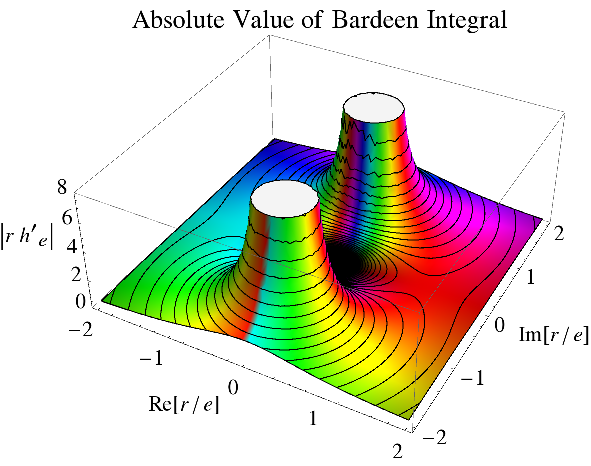
\includegraphics[width=\linewidth]{plots/bardeen-3d.pdf}
            \caption{Absolute value on $z$-axis, argument as hue}
        \label{fig:bardeen-3d}
    \end{subfigure}
    \begin{subfigure}[b]{.50\linewidth}
        \centering
            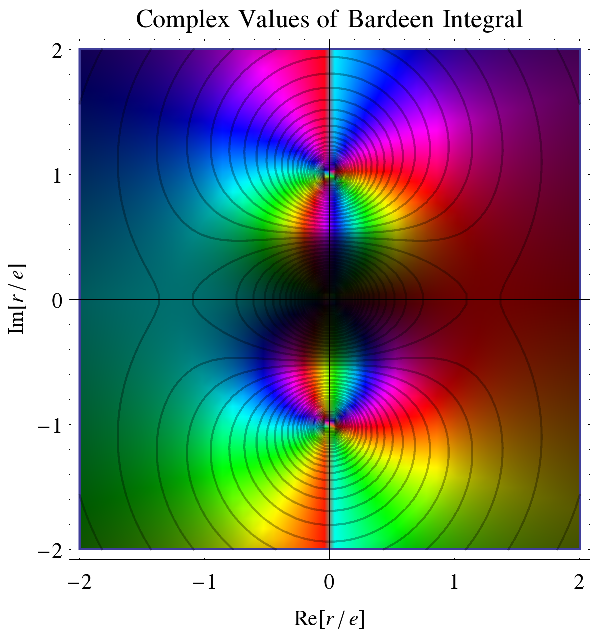
\includegraphics[width=\linewidth]{plots/bardeen-2d.pdf}
            \caption{Absolute value as brightness, argument as hue}
        \label{fig:bardeen-2d}
    \end{subfigure}
}
    \caption{The two essential singularities of the Bardeen integrand \eqref{eq:bardeen-v} are severe (wesentliche Singularität, kein Pol da $\nexists k \in \mathbb{N}: (z-z_0)^k v(z)$ hebbar {\it mit} $k$ minimal. Defakto $\exists k = \nicefrac 62$).
    }
    \label{fig:bardeen}
\end{figure}

\newpage
\section{The more general $h_\alpha$}
As said in the section before, the Bardeen solution is a special case of the self-regular Metric. In general it is given by \eqref{eq:halpha}. When setting (as derived in Calc7, Calc11 Section 2.2)
%
\begin{equation}
\alpha := \alpha_0 = \frac{3+n}{\ln (2+n)} \ln \frac{3+n}{2}
\end{equation}
%
then $h_{\alpha_0}$ shows the self-encoding radius property and $L$ is no more an arbitrary additional degree of freedom. Actually, the Bardeen solution is {\it not} self-regular, but shares the same form of equation.

I didn't consider the poles of $r^{1+n} h'_\alpha$ yet in any CalcX paper, so this will be caught up here.

\subsection{The $h_\alpha$ Poles}
The effective Function $v(r)$ to fourier-transform is
%
\begin{equation}
v(r) = r^{1+n}  \dd{h_\alpha(|r|)}{r} =
\frac{3+n}2
\frac{r^{1+n}}{\mathcolor{gray}{|r|^{2+n}}}
\frac{ L^\alpha |r|^{2+n} }
{ \left( \frac{L^\alpha}2 + r^\alpha \right)^
{\frac{3+n}\alpha + 1}
} \label{eq:halpha-generic}
\end{equation}
%
The obvious pole of eq \eqref{eq:halpha-generic} is
%
\begin{equation}
r_0 = \left( - \frac {L^\alpha}2 \right)^{\nicefrac 1{\alpha}}
= 2^{-1/\alpha} e^{i \pi / \alpha} L,
\end{equation}
%
but it is not the only one, due to the freedom of $\alpha$, there are plenty of others. It is uncomfortable (but possible, c.f. {\it Symmetrie für Bardeen.nb}, Section 1.1. {\it Die tatsächlichen Pole für beliebige $\alpha$ und $n$}) to write down all possible poles, dependent on $\alpha$ and $n$.

Symmetry discussions about $v(r)$ lead to a bunch of plots, c.f. figure \ref{img:halpha-poles}.

%The issue with $r<0$ must be considered for generic $h_\alpha$, because \eqref{eq:halpha-generic} is no more odd/even, compared to the Bardeen case. Actually, there is another superficial pole at $r_0 = -2^{1/\alpha} e^{i\pi/\alpha} L$ which apparently can be found by point reflection at $r=0$ in the complex plane (ist wahrscheinlich falsch: Lediglich Achsenspiegelung). This is discussed a bit in the Appendix section \ref{appendix:fourierN} or also in {\it Symmetrie für Bardeen.nb}.

\subsection{The self-encoding Poles}
When we fix $\alpha:=\alpha_0$ for the self-encoding property, it is more reasonable to really denote all poles. Working in dimensionless $z=r/L$, the number of poles $|P_{v(r)}|$ can now be expressed merely in terms of $n$:
%
\begin{equation}
|P_{r^{1+n} h'_{\alpha_0}(r)}| = (2,2,4,4,4,6,6,8) \quad \text{for } n=0..7
\end{equation}
%
The numeration and including is given by the shape of $v_\pm(r) = r^{1+n} h'(\pm r)$. That is, when writing in the spirit of \eqref{eq:f7}
%
\begin{align}
\C A^{-2}(p) &= \frac{2\pi i}p \int_{-\infty}^\infty \d r~ 
\frac{ r^{1+n} }{\mathcolor{gray}{|r|^{2+n}}}
\left( h'_{\alpha_0}(-r)~\Theta(-r) + 
h'_{\alpha_0}(r)~\Theta(r) \right) ~e^{-ipr} \\
&= \frac{2\pi i}p \int_{-\infty}^\infty \d r~ \left( v_{\bf -}(r)~\Theta(-r) + v_{\bf +}(r)~\Theta(+r) \right)~e^{-ipr}
\end{align}
%
Then the Cauchys Theorem can be applied for the roots of $v_{\bf -}(r)$ and $v_{\bf +}(r)$ (or $-$ for {\bf L} and $+$ for {\bf R} for {\it left} and {\it right} side of the complex plane). See figure \ref{img:halpha-poles}.

\vspace{2cm}
\subsection{The evaluated Integral ($\alpha_0$)}
It is pure coincidence that at least for $n \in \{0,1,\dots,7\}$ no pole of $v_\pm(r)$ is on $\text{Im}(r)=0$ or on $\text{Re}(r)=0$. So the whole procedure should be well-defined. See figure \ref{img:halpha-poles} for a plot of all singularities.

Nevertheless, the Residuum is not well defined. This is the same situation as for Bardeen (figure \ref{fig:bardeen}). The Laurent series at the pole positions do not converge, therefore a Residuum cannot be given. Only for $n=0$, the result is trivially 0 because there is no pole. This special case highlights another problem, because the Fourier Transform of the 4d Holographic Model is most likely not vanishing. Does this indicate that the complete calculation is not applicable?

For example, consider $n=1$. As plotted in figure \ref{img:halpha-poles}, there are two poles, $z_\pm = \pm 3^{-\frac{1}{4}+\frac{i \pi }{4 \log (2)}}$. When trying to taylor $v_R$ at $z_+$, we encounter diverging terms. This is because (for illustration)
%
\begin{equation}
v'_R(r/L)  = -\frac{4 r^4 \left(r^{\alpha }+\frac{1}{2}\right)^{-4/\alpha } \left(2 \alpha  r^{\alpha }-2 r^{\alpha
   }-5\right)}{\left(2 r^{\alpha }+1\right)^2}
\end{equation}
%
has even higher powers, so $v'_R(z_+)$ diverges. This is even more serious at higher orders.

\clearpage
\section{The holography model, revisited}
The holographic model
%
\begin{equation}
h(r) = \frac{r^{2+n}}{r^{2+n} + L^{2+n}}
\end{equation}
%
was the first one which I tried to Fourier transform. While my first try was rather CAS assisted, I know performed pole summing, that is, regular Cauchy Theorem. Actually, figure \ref{img:holo-poles} shows the poles of
%
\begin{equation}
v_\pm(r) = \frac{r^{1+n}}{\mathcolor{gray}{(\pm r)^{2+n}}}
\frac{L^{2+n} (2+n) (\pm r)^{1+n}}
{ \left(L^{2+n} + (\pm r)^{2+n} \right)^2 }
\end{equation}
%
Solutions get quickly very complex. Only $n=0$ one can write it in one line:
%
\begin{equation}
\C A^{-2}(p) \propto -2\pi e^{-p} + \frac{ 2\pi e^{-p}}p
\end{equation}
%
Figure \ref{img:holo-a} plots the Real and Imaginary parts for $n=0..7$. The curves look somewhat promising, but this probabily changes dramatically if one computes $\left( \C A^{-2}(p) \right)^{-1/2}$.

% Doch nicht wahr, da diese Pole jeweils zum anderen R/L gehoeren!
%Furthermore, I slightly ignored a serious problem which can be spotted in figure \ref{img:holo-poles} for $n=1,3,5,7$: There are poles $r=\pm1$, which is straight on the integration contour. Is there any reason why one could choose an integration countour around these poles? If so, which way 

\begin{figure}
\center
\makebox[\textwidth][c]{
	\centering
	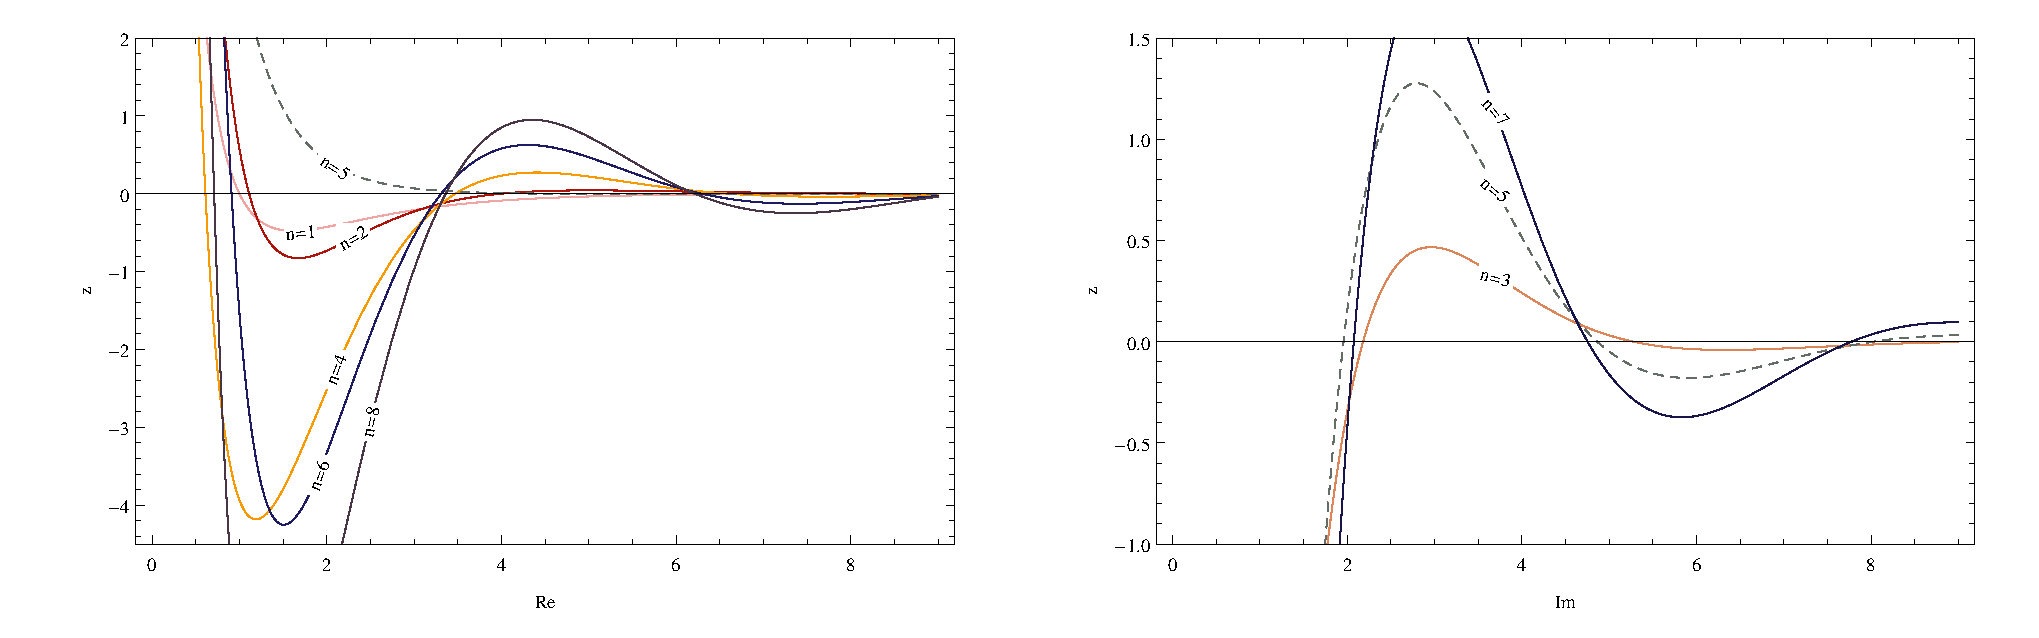
\includegraphics[width=1.25\textwidth]{plots/holo-A.pdf}}
\caption{$\C A^{-2}(p)$ for Holographic Function. $n=0$ is Real and to small to be visible, but behaves like $n=1$. $n=5$ is special because it has both Re and Im. Defacto these plots lack another imaginary $i$ prefactor and perhaps an axis scaling (c.f. Appendix \ref{section:appendix-dimensionless}), but this doesnt change the nature of the curves.
 } \label{img:holo-a}
\end{figure}


\begin{figure}
\center
\makebox[\textwidth][c]{
	\centering
	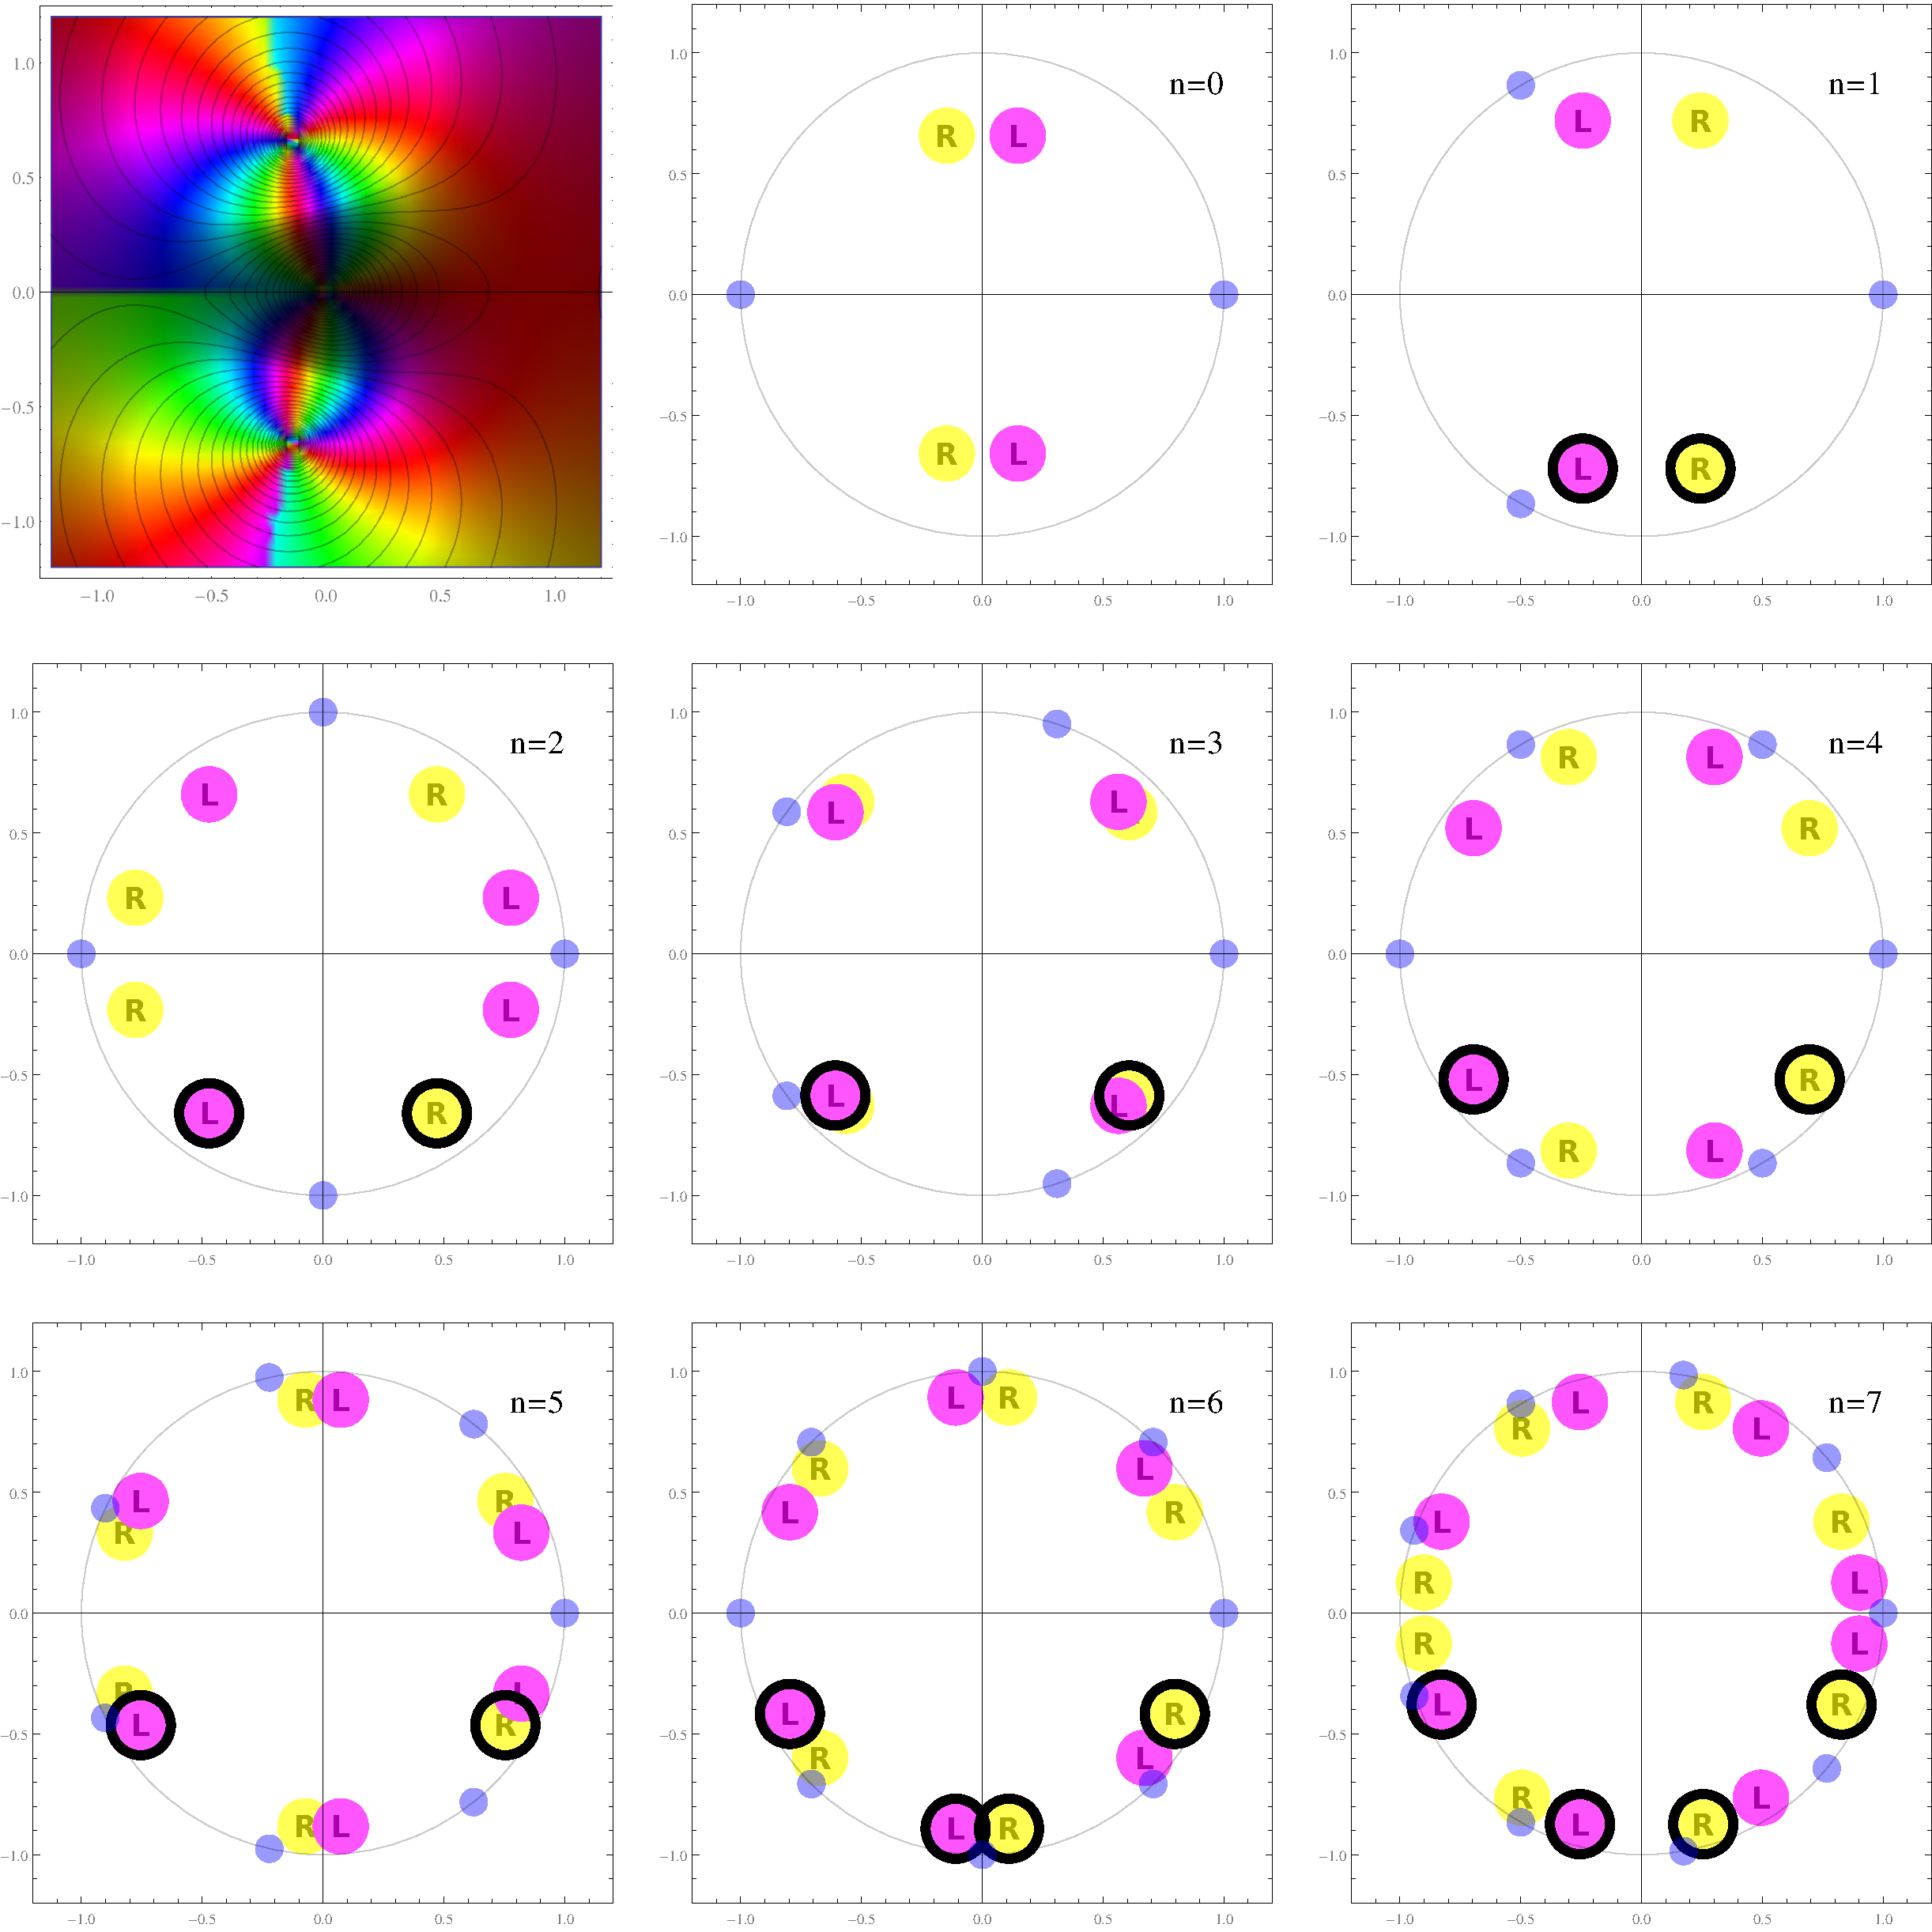
\includegraphics[width=1.15\textwidth]{plots/halpha-poles2.pdf}}
\caption{The poles of $v_{\bf L}(r) = r^{1+n} h'_{\alpha_0}(-r)$ and
$v_{\bf R}(r) = r^{1+n} h'_{\alpha_0}(+r)$ for different dimensions $d=3+n$ in the complex plane. Encircled poles can be take into account for Cauchys theorem.  The small blue circles on the unit sphere indicate the $n+2$. root of unity. The upper left panel shows a complex plot of $v_{\bf L}$ for $n=0$ (c.f. figure \ref{fig:bardeen-2d}). Therefore the first panel shows a subset of the second panel. As one can see, $n=0$ is a special case where there is no pole in the integration area.
 } \label{img:halpha-poles}
\end{figure}

\begin{figure}
\center
\makebox[\textwidth][c]{
	\centering
	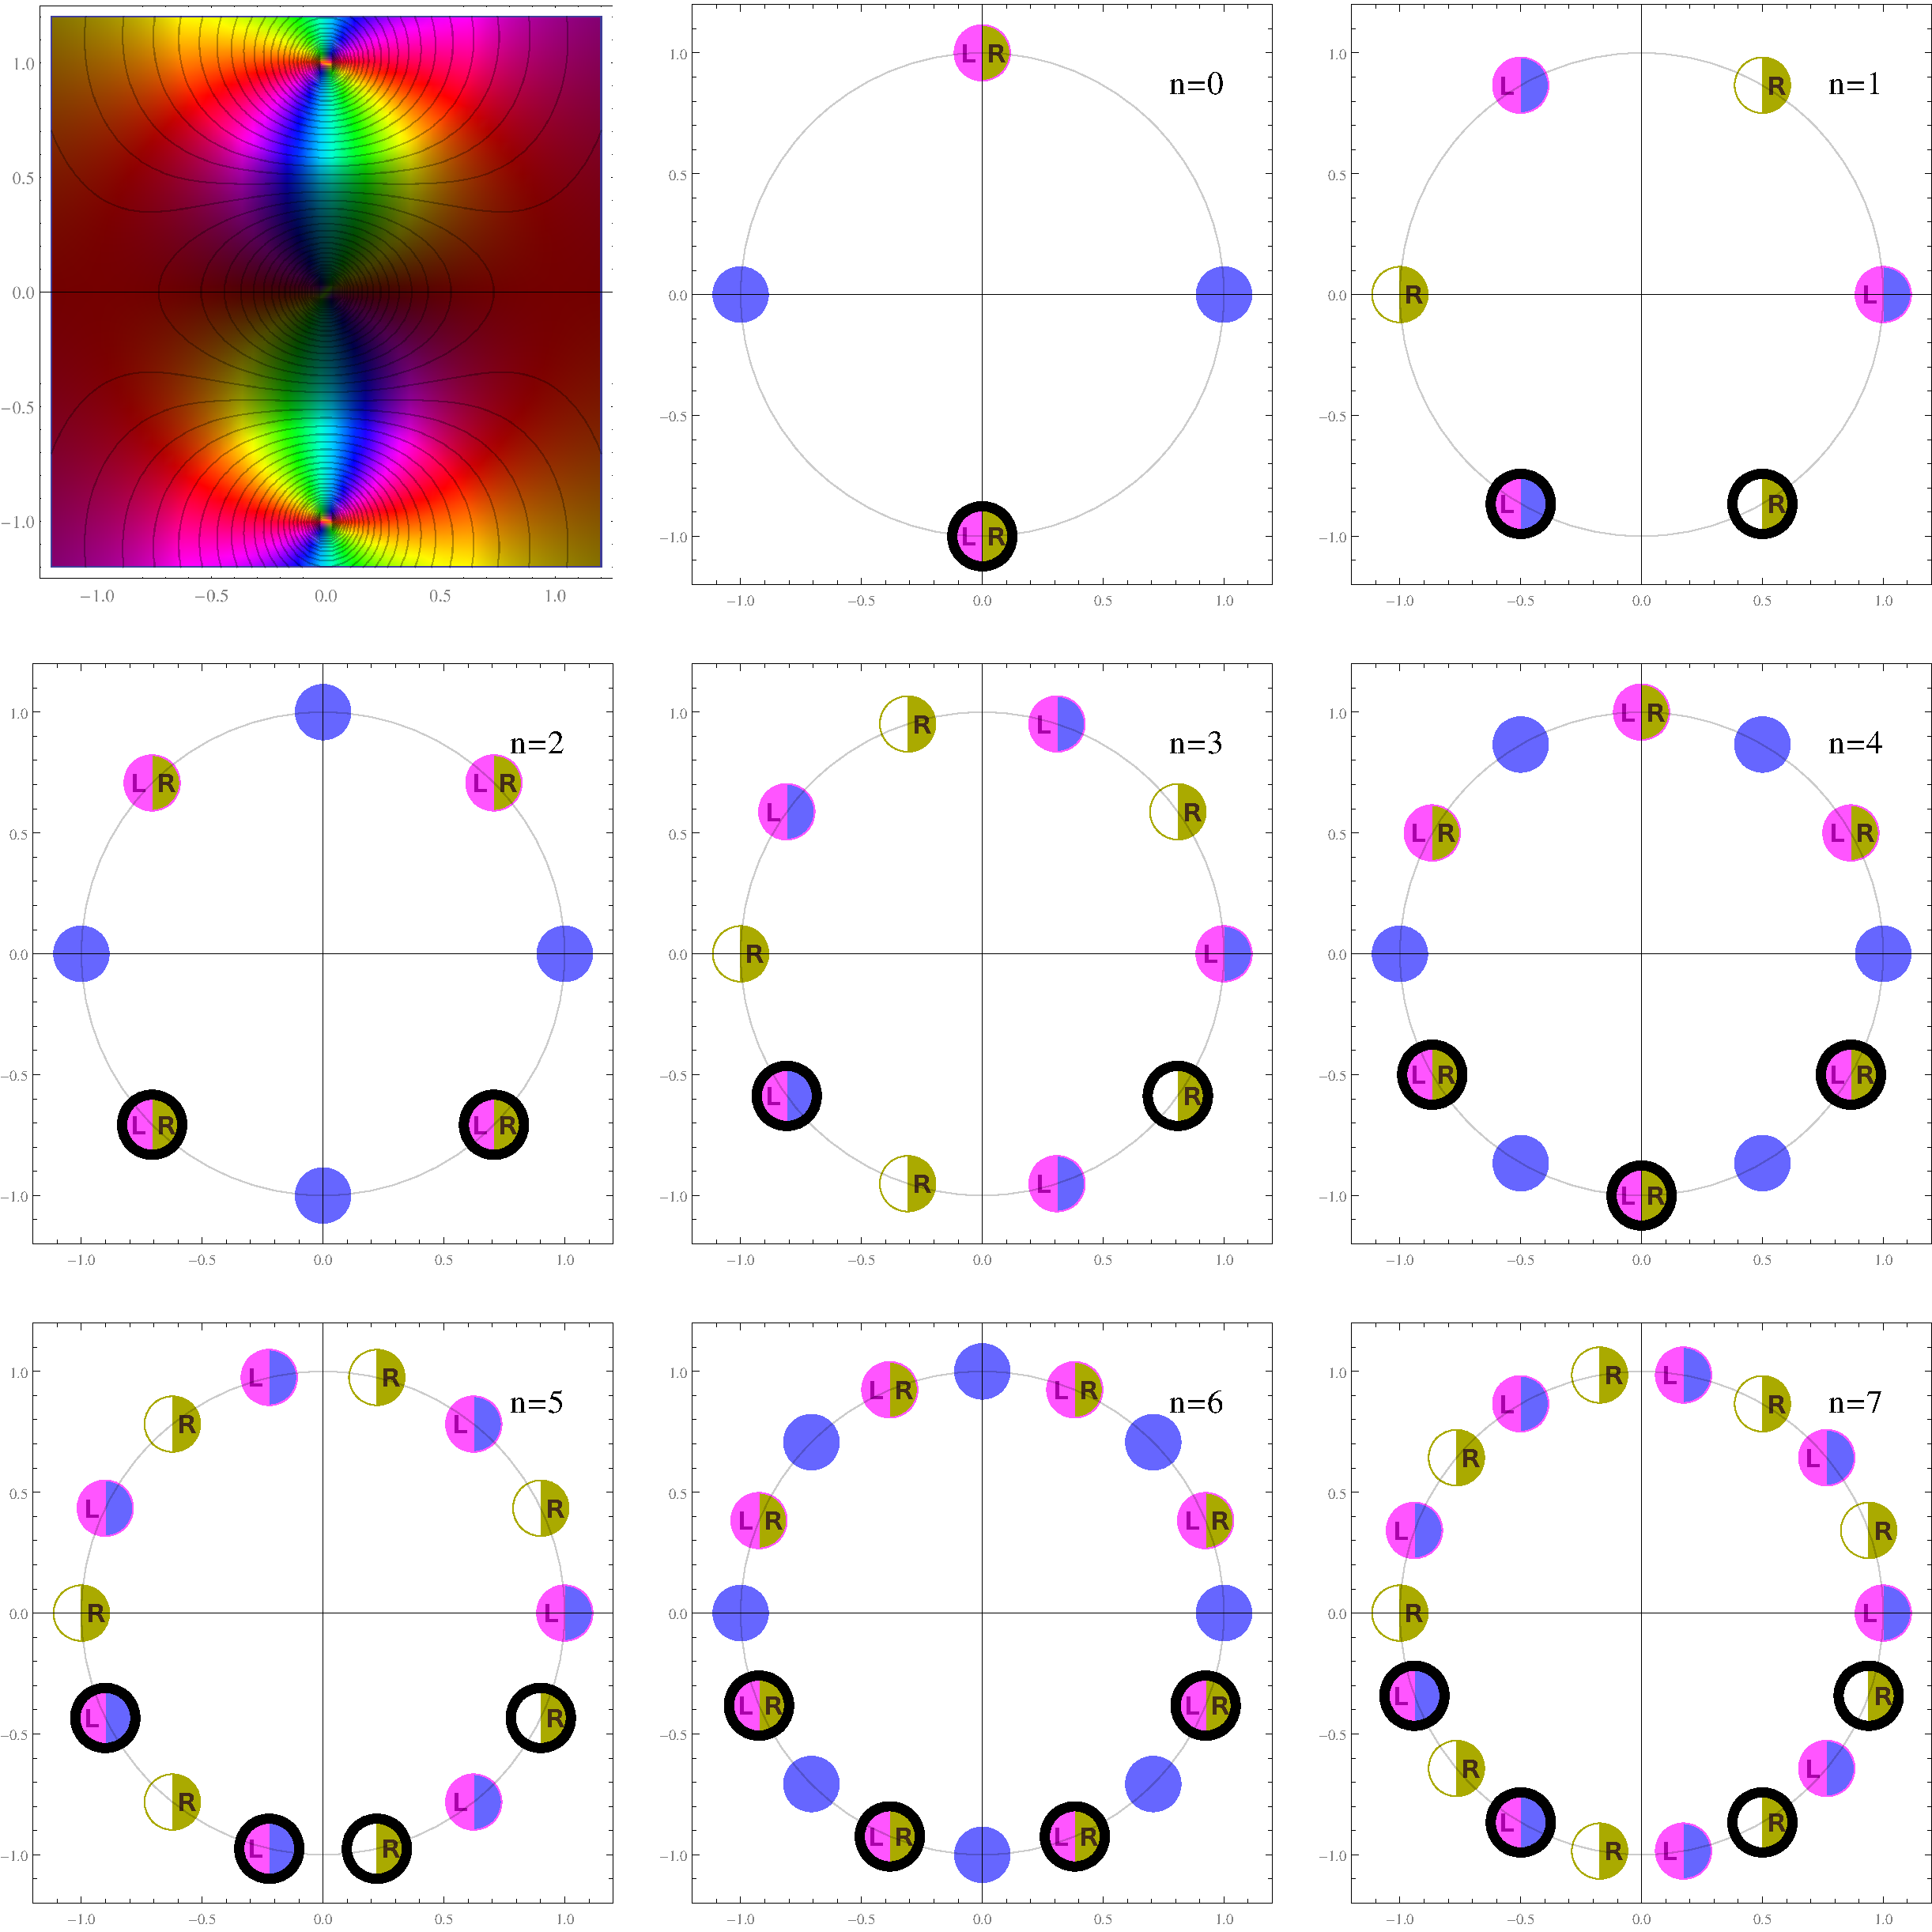
\includegraphics[width=1.15\textwidth]{plots/holo-poles.pdf}}
\caption{The poles of Holographic Function Integration kernel $v_\pm(r) = r^{1+n} h'(\pm r)$ in $n$ dimensions. Same conventions used as in figure \ref{img:halpha-poles}.
\\
Note the poles on $r=\pm1$ for $n=1,3,5,7$. They are straight on the integration contour, but do not count because in all cases, $R$ and $L$ are on the wrong side. That was close!
 } \label{img:holo-poles}
\end{figure}


\newpage
\begin{appendices}
\section{Verification Strategies}
\begin{itemize}
 \item {\bf Searching the Poles}: Analytic result (Solve/Reduce) {\it vs.} 3d Plots like figure \ref{fig:bardeen}.
 \item {\bf Performing the FT}: Cauchy Theorem (Summation of Poles) {\it vs.} Numerical evaluation of Integral, see Appendix \ref{section:appendix-dft}.
\end{itemize}

\section{Review of the radial symmetric $d$-dimensional FT} \label{appendix:fourier}
This calculation was already performed in Calc10, section 1.1.1, but not in detail. Actually I always thought, a minus was missing there. Let's review it.

In the end I want to use the the Fourier transformation $\C F$ which is defined in $d$ dimensions ($\vec x \in \mathbb R^d$) as
%
\begin{subequations}
\begin{align}
\C F\left\{ f \right\}(\vec p) &= \tilde f(\vec p) = \frac 1{(2\pi)^d} \int \d^d x~e^{-i\vec p \cdot \vec x} f(\vec x) \label{eq:Four1} \\
\C F^{-1}\left\{ \tilde f \right\}(\vec x) &= f(\vec x) =   \int d^d p~e^{+i \vec p \cdot \vec x} \tilde f(\vec p) \label{eq:Four2}
\end{align}
\end{subequations}
%
For shortness of notation, I will supress the leading $(2\pi)^{-d}$ in the following equations.

We begin with $V=V(|\vec r|)$, a radially symmetric potential, and work at first in $d=3$ total spacial dimensions:

\begin{subequations}
\begin{align}
\hat V(p) &= \int \d^3 r ~e^{-i \vec r \cdot \vec p}~ V(r) \\
&= \int_0^\infty \d r \int_0^\pi r^2 \sin \theta ~ \d \theta \int_0^{2\pi} \d \varphi~V(r)~e^{-i p r \cos \theta_2} \label{eq:f2}
\intertext{In line \eqref{eq:f2} we already wrote the scalar product with an inner angle $\theta_2$. We now substitute the radial angle $\theta$ (the $\theta$ which is part of $\vec r = (r,\theta,\varphi)$) integration with a $\cos \theta$ integration. This can be done because $\dd{\cos \theta}\theta = -\sin \theta$ and so $\int_0^\pi \sin \theta \d \theta = -\int_{-1}^1 \d \cos \theta = \int_{-1}^1 \d \cos \theta := \int_{-1}^1 \d x$. We now identify $\cos \theta := x$ with $\cos \theta_1$ because they share the same domain, actually $\theta,\theta_1 \in \{0,\pi\}$. We continue (naturally, $\int_0^{2\pi}\d \varphi = 2\pi$ was already integrated out in the next line):
}
&= 2\pi \int_{-1}^{+1} \d x \int_0^\infty \d r ~r^2 ~e^{-i r p x} V(r) \\
&= 2\pi \int_0^\infty r^2 ~  \d r ~ V(r) \left[ \frac{1}{-ipr} e^{-iprx} \right]_{-1}^{+1} \\
&= \frac{2\pi i}p \int_0^\infty r~\d r~V(r) \left\{ e^{-ipr} - e^{+ipr} \right\} \\
&= \frac{2\pi i}p \left\{ \int_0^\infty r~\d r~V(r) e^{-ipr} - \int_0^\infty r~\d r~V(r) e^{+ipr} \right\} \label{eq:f3}
\intertext{In line \eqref{eq:f3}, we splitted the integral, and we now make two recastings: At first, switching the integral borders, which inserts one \textcolor{red}{minus}: $\int_a^b = \redmin \int_b^a$ in \eqref{eq:f4}. Second, another substitution of the integration parameter $r:=\redmin r'$ and therefore $\d r = \redmin \d r'$. The two minus signs kill each other in \eqref{eq:f5}, so $r \d r = r' \d r'$. After substitution, we will call $r'$ again $r$, which is totally valid.
}
&= \frac{2\pi i}p \left\{ \int_0^\infty r~\d r~V(r) e^{-ipr} \redplus \int_{\infty}^0 r~\d r~V(r) e^{+ipr} \right\} \label{eq:f4} \\
&= \frac{2\pi i}p \left\{ \int_0^\infty r~\d r~V(r) e^{-ipr} \redplus \int_{\redmin \infty}^0 r'~\d r'~V(\redmin r') e^{\redmin i p r'} \right\}  \label{eq:f5} \\
&= \frac{2\pi i}p \int_{-\infty}^\infty r~\d r~ e^{-ipr}~
\left\{ V(r) \Theta(r) + V(-r) \Theta(-r) \right\} \label{eq:f6} \\
&= \frac{2\pi i}p \int_{-\infty}^\infty \d r~ \left\{ r V(|r|) \right\}~e^{-ipr} \label{eq:f7}
\end{align}
\end{subequations}
Basically \eqref{eq:f7} is our final result. The more extensive eq. \eqref{eq:f6} may be better to argue why I think the new {\it effective} one dimensional function $v(r)\sim r~V(|r|)$ can still be treated as a holomorphic function, because all this work is about smearing the $\Theta$, so it is no more a special distribution. Probabily, since our functions $V(r)$ don't have poles at $r=0$, the discontinuity issue at $r=0$ may be silently ignored, reasoning that it is always possible to let $V(-r)$ and $V(r)$ blend into each other in a continous way.

Whats about the real and complex parts of this fourier transformation? By construction, $V(|r|)$ is an even function (definition: $f(x)=f(-x)$ is even, $-f(x)=f(-x)$ is odd). Therefore $r~V(|r|)$ is an odd function. By eulers formula $e^{i\varphi} = \cos \varphi + i \sin \varphi$, one quickly finds that the Fourier Transform of an even function includes only (also even) $\cos$ terms and the complex part vanishes, while the FT of an odd function only contains $\sin$ terms and the real part vanishes. The integral in \eqref{eq:f7} is therefore ony complex, $\int \d r~rV(|r|)e^{-ipr} \in \mathbb{C} \setminus \mathbb{R}$. But the prefactor makes the final result in \eqref{eq:f7} completely real again. This can help as a quick check wether the computed result of the integral is correct.

% So ignoring the $\Theta$ issue, there is a general guide how to solve \eqref{eq:f7}: We can use Cauchy theorem, and because $p=|\vec p|>0$, we always close the integration path at $r=-i\infty$ because then $e^{-ipr}\to e^{-i(+\#)(-i\infty)} = e^{-\# \infty} \to 0$. We only consider the poles $r_0$ in the region $(\text{Re } r_0 > 0 \land \text{Im } r_0 < 0)$ (IV. quadrant in two dimensional Cartesian coordinate system). We mirror them at the $y$ axis, which means effectively two count every pole {\it two (more) times}, because $V(|-r|)=V(|r|)$ ({\bf Das ist wahrscheinlich falsch! Denn $-r V(|-r|) \neq r V(|r|)$!! Das Ergebnis ist dann Null}).

\subsection{From 3 to (3+n) dimensions} \label{appendix:fourierN}
The same calculation can be performed in $d=3+n$ spatial dimensions. It is easy to derive then the pendant of \eqref{eq:f7} as (TODO not sure about $\Omega$, to be checked)
%
\begin{equation}
\hat V(p) = \Omega_{2+n} \frac{i}p \int_{-\infty}^\infty \d r~ r^{1+n} V(|r|)~e^{-ipr}  \label{eq:f7.2}
\end{equation}
%
The symmetry of the effective function $v(r)\sim r^{1+n}~V(|r|)$ now dramatically depends on $n$. Actually, for even $n=0,2,4,\dots$, $v(r)$ is odd, where for odd $n=1,3,5,\dots$, $v(r)$ is even. Figure \ref{fig:fourier-even} shows this on an arbitrary function $V(|r|)$.

\begin{figure}[h]
\center%
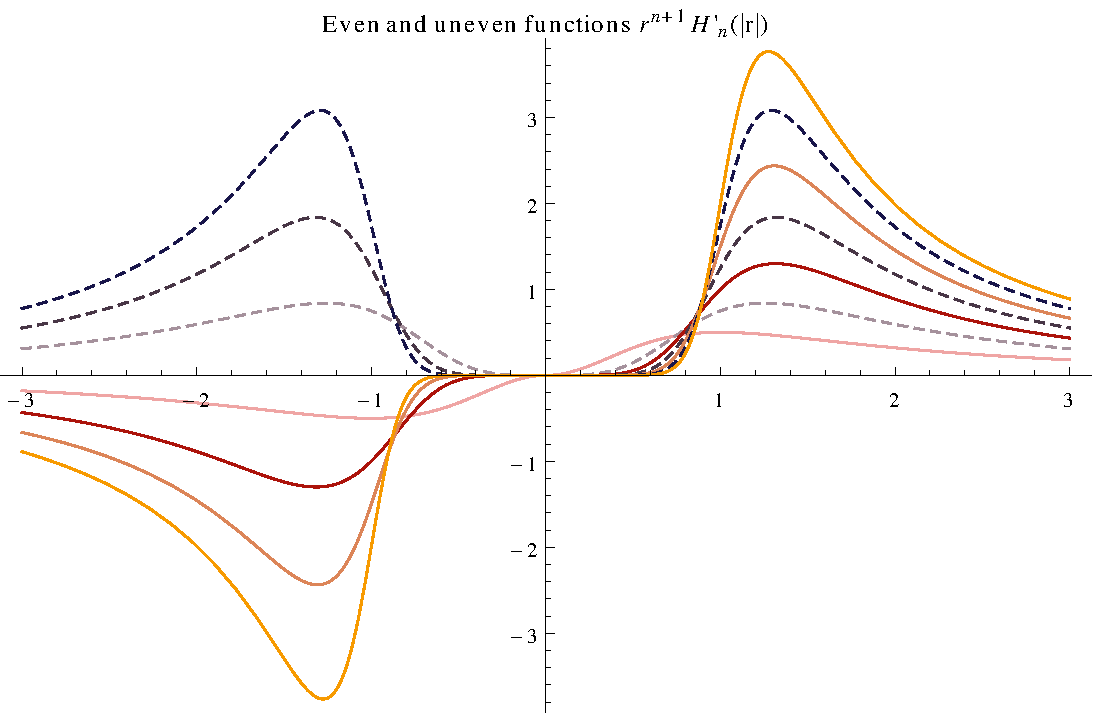
\includegraphics[width=13cm]{plots/fourier-even.pdf}
\caption{Dashed lines represent symmetric (even) functions $v(r)$ and thus belong to $n=1,3,5$. Solid lines belong to $n=0,2,4$. Here, $V(|r|)=h'_n(|r|/L) = \partial_r \left(r^2 / (r^2 + 1) \right)_{r\to |r|}$
}\label{fig:fourier-even}
\end{figure}

In consequence, this means for the Fourier Transformation in $(n+3)$ dimensions,
\begin{equation}
\C F_{n+3} \left\{ V(|r|) \right\} \in 
\begin{cases}
\mathbb{C} \setminus \mathbb{R}   &\mbox{if } n \in \{ 1,3,5, \dots \} \\
\mathbb{R}   &\mbox{if } n \in \{0,2,4,\dots \}
\end{cases}
\end{equation}

Furthermore, \eqref{eq:f7.2} allows us to use Cauchy theorem to solve all $\C F_{n+3}$. Since $p=|\vec p|>0$, we always close the integration path at $r=-i\infty$ because then $e^{-ipr}\to e^{-i(+\#)(-i\infty)} = e^{-\# \infty} \to 0$. We therefore sum over all poles $r_0$ in the region $\text{Im} r_0 < 0$. Poles in the region $(\text{Re } r_0 > 0 \land \text{Im } r_0 < 0)$ (IV. quadrant in two dimensional complex plane) can be determined by solving the equation $r^{-(1+n)}/V(r) = 0$ (and ignoring all poles outside the target region), where poles in the region $(\text{Re } r_0 < 0 \land \text{Im } r_0 < 0)$ can be determined with $r^{-(1+n)}/V(-r) = 0$ (same applies here). I'm not sure yet if mirroring at the $y$ axis, which means effectively two count every pole {\it two (more) times} is also valid.

\subsection{Dimensionless calculation} \label{section:appendix-dimensionless}
To simplify calculation, I frequently use dimensionless $z=r/L$ ($L > 0$) when working with functions $V(r)=V(z)$. Having $\d r = L \d z$ and $\dd{f(r)}{r} = \dd{f(r)}z \dd zr = \frac 1L \dd{f(z)}r$, the integral
%
\begin{equation}
\int_{-\infty}^{\infty} \d r \dd{H(r)}{r}
= \int_{-L\infty}^{L \infty} \d z \dd{H(z)}{z}
\end{equation}
%
does not change under transformation. But there are other factors. Consider again \eqref{eq:f7.2}. By inserting $q=L p$, the transformation does not change the shape of the integral:
\begin{subequations}
\begin{align}
\hat V(p) &= \Omega_{2+n} \frac{i}p \int_{-\infty}^\infty \d r~ r^{1+n} V(|r|)~e^{-ipr} \\
&= \Omega_{2+n} \frac{i}{p} L^{1+n} \int_{-\infty}^{\infty} \d z~z^{1+n} V(|z|) e^{-i q z} \\
&= L^{n} \left( \Omega_{2+n} \frac{i}{q} \int_{-\infty}^{\infty} \d z~z^{1+n} V(|z|) e^{-i q z} \right)
:= L^n \hat V_z(q)
\end{align}
%
So for comparing the graphs of the dimensionless quantity $\hat V_z(q)$ with the dimensionful, the mapping is given by
%
\begin{equation}
\left( p, \hat V(p) \right)
= \left( q / L, L^n \hat V_z(q/L) \right)
\end{equation}
\end{subequations}

\newpage
\section{$d$-dimensional discretized FT} \label{section:appendix-dft}
These calculations are inspired by numerical physics computations, as they are done e.g. in Lattice QCD. We start with a simple one dimensional example.

Let $\vec r=(r)$ be the one dimensional position space vector. Working in a box (or on a finit one dimensional number line) with $N \in \mathbb{N}$ distinct elements (spacial extend of the box), we discretize $r=n~a$ with $n \in [0,N-1]\setminus\mathbb{N}$ and the lattice spacing $a$ which has the physical unit $[a]=L$.

On such lattice with a spacing $a$, the minimum wave length (and therefore the maximal momenta) is $\frac{2\pi}a$. The momentum is therefore discretized following $p=\frac{2\pi k}{a~N}$ with $k\in[0,\frac{2\pi}a]\setminus\mathbb{N}$.

With these conventions, the transition from the analytic Fourier Transformation to the Discrete Fourier Transform (DFT, not to be confused with the Fourier Series) can be archived. Lets start with the one dimensional

\begin{subequations}
\begin{align}
\hat f(p) &= \int_{-\infty}^{\infty} f(r)~e^{-i p r}~\d r \\
\intertext{At first, we make the infinities finite, so $\int \d r \to \sum \Delta r$. Due to the boxing, $\sum\limits^{\infty} \to \sum\limits^N$. In the limes, this process is well-defined.
}
&= \lim_{\Delta t \to 0} \sum \Delta t ~ f(r)~e^{-ipr} \\
&= \lim_{\Delta t \to 0} \Delta t \sum_{n=0}^N f(an)~ e^{-i \left( \frac{2\pi k}{aN}\right) a~n} \\
&= \lim_{\Delta t \to 0} \Delta t \sum_{n=0}^N f(an)~ e^{-\frac{2\pi i}N kn}
\end{align}
\end{subequations}
%
We end up with the definition of the DFT. When we treat functions as lists, $f(an)\to f_n$ and $\hat f(p)\to f_k$, we can compute Fourier Transformations of lists.

Caution has to be taken when comparing DFT and ordinary FT results, both in respect to the prefactors and the $p$ scaling. E.g. {\it Mathematica} defines these operations as
\begin{subequations}
\begin{align}
{\tt FourierTransform[}f(t),t,\omega{\tt ]} &= \frac{1}{\sqrt{2\pi}} \int_{-\infty}^\infty f(t)~e^{\redplus i\omega t}~\d t \\
{\tt Fourier[}\{u_r\}{\tt ]} = \{ v_s \} &= \frac{1}{\sqrt N} \sum_{r=1}^N u_r~e^{\redplus \frac{2\pi i}N (r-1)(s-1)}
\quad\text{with }N=|\{ u_r\}|=|\{v_s\}|
\end{align}
\end{subequations}
%
which means identifying the graphs $(x,f(x))$ of these equations requires (using again $n,k=r,s$)
%
\begin{equation}
\left(\frac{2\pi k}{a N}, \sqrt\frac{2\pi}N \hat f_k \right) = (p, \hat f(p))
\label{eq:apxC-1}
\end{equation}
%
Actually, althought I investigated two or three days of work to examine numerical evaluation of the Transformation, in the hope of a simple comparison between analytical and numerical results from \eqref{eq:apxC-1}, this was not possible yet. Perhaps my lattice was too small -- the results were only suitable as a very bad approximation.

\end{appendices}
\end{document}
